\documentclass[conference]{IEEEtran}
\usepackage{iftex}
\ifXeTeX\usepackage{fontspec}\setmainfont{texgyretermes-regular.otf}[BoldFont=texgyretermes-bold.otf,ItalicFont=texgyretermes-italic.otf,BoldItalicFont=texgyretermes-bolditalic.otf]\fi
\usepackage{graphicx}
\usepackage{booktabs}
\usepackage{amsmath}
\usepackage{url}
\usepackage{tikz}
\usepackage{pgfplots}
\pgfplotsset{compat=1.16}
\usetikzlibrary{arrows.meta,positioning,shapes.geometric}

\begin{document}

\title{Portlogi: A Departure-Aware Digital Twin for Container Yard Placement and Truck Booking at Indian Ports}

\author{\IEEEauthorblockN{Harsha Vardan M Sakamuri and Akshathra Selvam}
\IEEEauthorblockA{VIT Chennai, Tamil Nadu, India}}

\maketitle

\begin{abstract}
In a container yard, a box that sits on top of another box that leaves earlier causes an extra lift, called a rehandle. Rehandles waste vehicle time and make trucks wait at the gate. At Indian ports the problem is made worse by long dwell times and by pickup times that are mostly unknown when a box is placed. This paper describes Portlogi, a simulated smart yard for V.~O. Chidambaranar Port, Thoothukudi. It admits a box when its RFID card is read, picks a slot with hard safety rules and a five part score, moves boxes with several self driving vehicles that never share a cell, and lets a business book a truck so the yard learns the pickup time. On a small yard, the allocator cut rehandles by 69.6\% against first available placement (6.7 to 2.0 per 30 boxes, 100 runs). Against a rule that already uses departure times it cut them by about 31\%. A second experiment shows that a pickup time only reduces rehandles if it is known when the box is placed, while a later booking still removes truck waiting. No safety rule was broken in 200 random yards. The site is hosted on AWS and scored A+ on two public security scans. All results come from simulation. The RFID gate hardware is planned and not yet built.
\end{abstract}

\begin{IEEEkeywords}
container yard, rehandling, digital twin, smart port, truck booking, RFID
\end{IEEEkeywords}

\section{Introduction}
Ports are the doors of a city's economy. Containers come off a ship, wait in a yard, and leave by truck or rail. The yard stacks containers to save space. Stacking has a cost. If the box you need is under another box, the top box must be lifted away first. That extra lift is a rehandle.

Time in the yard is long in India. A report on the first quarter of 2024 says the median export dwell time rose to more than four days, up from about three and a half days a year earlier \cite{bw2024}. Long stays mean full yards, and full yards mean more rehandles. There is another problem. The yard has to place an import box before it knows when a truck will come for it. Without a pickup time, the best placement is a guess.

The Tamil Nadu Smart Cities project covers Thoothukudi, home of V.~O. Chidambaranar (VOC) Port. The port handled 734,274 TEU in 2022-23 \cite{wikivoc}. We chose it as the setting for a smart yard that is also a service for businesses. In that service, the port authority offers a booking desk to shipping lines and hauliers. This is the government to business (G2B) idea.

\textbf{Objectives.} (1) Place each box so it is unlikely to block another. (2) Move boxes with several vehicles without collisions. (3) Let a business book a truck so the yard learns the pickup time. (4) Show the reason for every decision and replay any run exactly. (5) Offer the system over a secure web link.

\textbf{Contribution.} We built a working simulator with these parts and measured it. We also ran an experiment that asks what a pickup time is worth, and when it must arrive.

\section{Literature Review}
Container stacking with departure information is a known topic. Dekker et al. studied stacking policies by simulation and showed that using departure times lowers rehandles \cite{dekker2006}. Caserta et al. proved the blocks relocation problem is hard and gave exact and rule based methods \cite{caserta2012}. Ku and Arthanari looked at the case where departure times come as time windows, for example from a truck appointment system, and built a model and a fast heuristic for it \cite{ku2016}. Galle et al. studied the stochastic version, where the retrieval order is uncertain \cite{galle2017}.

For vehicle traffic, Mohring et al. describe conflict free routing of automated guided vehicles (AGVs) by time windows, tested at a Hamburg terminal \cite{mohring2005}. Kim, Jeon and Ryu study how deadlocks form between AGVs and how to prevent them \cite{kim2007}. On the product side, a vendor reports a 25\% drop in rehandles after a yard planning tool went live at one terminal \cite{kaleris2023}. In India, the Logistics Data Bank tracks containers with RFID tags \cite{ldb}.

\begin{table}[t]
\caption{What each line of work covers}
\label{tab:related}
\centering
\small
\begin{tabular}{lcccc}
\toprule
Work & Stacking & Uncertain & Traffic & Booking \\
 & by time & time & control & desk \\
\midrule
Dekker et al. \cite{dekker2006} & yes & no & no & no \\
Ku and Arthanari \cite{ku2016} & yes & windows & no & no \\
Galle et al. \cite{galle2017} & yes & yes & no & no \\
Mohring et al. \cite{mohring2005} & no & no & yes & no \\
Kim et al. \cite{kim2007} & no & no & yes & no \\
This work & yes & yes & yes & yes \\
\bottomrule
\end{tabular}
\end{table}

\textbf{Gap.} We did not find a single open system that joins gate admission, placement, vehicle traffic and a business booking desk, with a replayable record of each decision. We also did not find a measurement of how the time a booking arrives changes the result. Table~\ref{tab:related} sums this up from the papers we read. It is not a full survey.

\section{Proposed Methodology}
Fig.~\ref{fig:arch} shows the plan. A card is read at the gate. The yard engine creates a container record and the allocator picks a slot. A vehicle is sent, a path is planned, and the move is done. For an import box, a business can book a truck. The booking sets the pickup time, and the yard brings the box to the gate before the truck is due.

\begin{figure}[t]
\centering
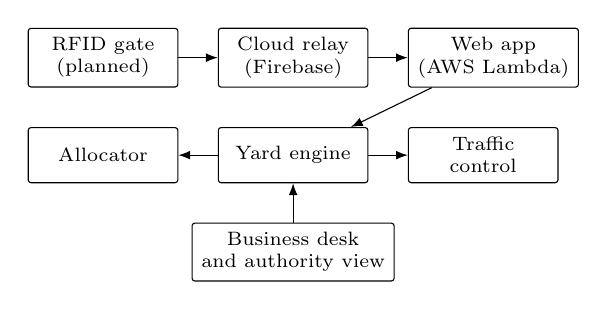
\begin{tikzpicture}[node distance=5mm and 5mm, every node/.style={font=\scriptsize}, box/.style={draw, rounded corners=1pt, minimum width=1.9cm, minimum height=0.7cm, align=center}, arr/.style={-{Latex[length=1.5mm]}}]
\node[box] (gate) {RFID gate\\(planned)};
\node[box, right=of gate] (cloud) {Cloud relay\\(Firebase)};
\node[box, right=of cloud] (app) {Web app\\(AWS Lambda)};
\node[box, below=of cloud] (eng) {Yard engine};
\node[box, left=of eng] (alloc) {Allocator};
\node[box, right=of eng] (traffic) {Traffic\\control};
\node[box, below=of eng] (desk) {Business desk\\and authority view};
\draw[arr] (gate) -- (cloud);
\draw[arr] (cloud) -- (app);
\draw[arr] (app) -- (eng);
\draw[arr] (eng) -- (alloc);
\draw[arr] (eng) -- (traffic);
\draw[arr] (desk) -- (eng);
\end{tikzpicture}
\caption{System plan. The gate hardware is planned. The other parts are built.}
\label{fig:arch}
\end{figure}

\subsection{Placement}
Each free slot is first checked against hard rules. A reefer needs a powered slot. A heavy box may not sit on a lighter one. A hazardous box may not touch another hazardous box. Slots that pass are given a score, and the lowest score wins:
\begin{equation}
C(s)=40\,r+15\,t+15\,c+12\,p+18\,a
\end{equation}
Here $r$ is rehandle risk (how much the box would sit on top of boxes that leave earlier), $t$ is the driving distance from the gate, $c$ is how well the box groups with ones for the same destination, $p$ is how much the yard would spread into fresh stacks, and $a$ is how much the slot would block the aisles. The numbers are weights, which the user can change. If no legal slot exists, the box waits on a transfer pad and is placed when a legal slot opens.

\subsection{Traffic}
Vehicles reserve cells for time windows along their path, so two vehicles never share a cell. A vehicle takes time proportional to the real distance of each segment, so it moves at a steady speed. If a ring of vehicles ends up waiting on each other, the system picks one by priority and sends it to a free cell until the ring clears.

\subsection{Booking}
An import box has no fixed pickup time. We guess that it leaves about 180 minutes after arrival, and mark the guess as false. When a business books a haulier and a window, the booking becomes the real pickup time. The yard then digs the box out if needed and brings it to the gate before the window. The booking desk shows a quote that includes the yard handling cost.

\section{System Design and Implementation}
\textbf{Software.} The engine is written in TypeScript. It is deterministic. Time moves in fixed ticks of 0.01 simulated minutes, and random numbers come from a seeded generator, so one seed always gives one result. Every user action is stored as a command in a journal, and the journal can replay a run exactly. Safety checks run during the simulation. They test that no two vehicles are closer than a set distance, that every stack is legal, and that no box is lost or doubled. The interface uses React and runs in a browser. Heavy comparisons run in a web worker.

\textbf{Hardware (planned).} An ESP32 board with an RFID reader will send the card number to a cloud database. The database rules let a gate device add scan records only. Reading needs a sign in, and public sign up is off. The page then admits the box. This part is written but has not been tested with real hardware.

\textbf{Hosting.} The site runs on AWS Lambda behind a secure web link. The response headers set a strict content security policy and other protections. A script checks the live site against 31 rules, and each deploy first checks that only free tier services are used.

\textbf{Ports.} A landing page shows an OpenStreetMap map \cite{osm} with 17 Indian ports. Each port opens its own illustrative yard with its own size, stack height, vehicles and settings. These yards are made up for the demo. The real layouts were not found.

\begin{figure}[t]
\centering
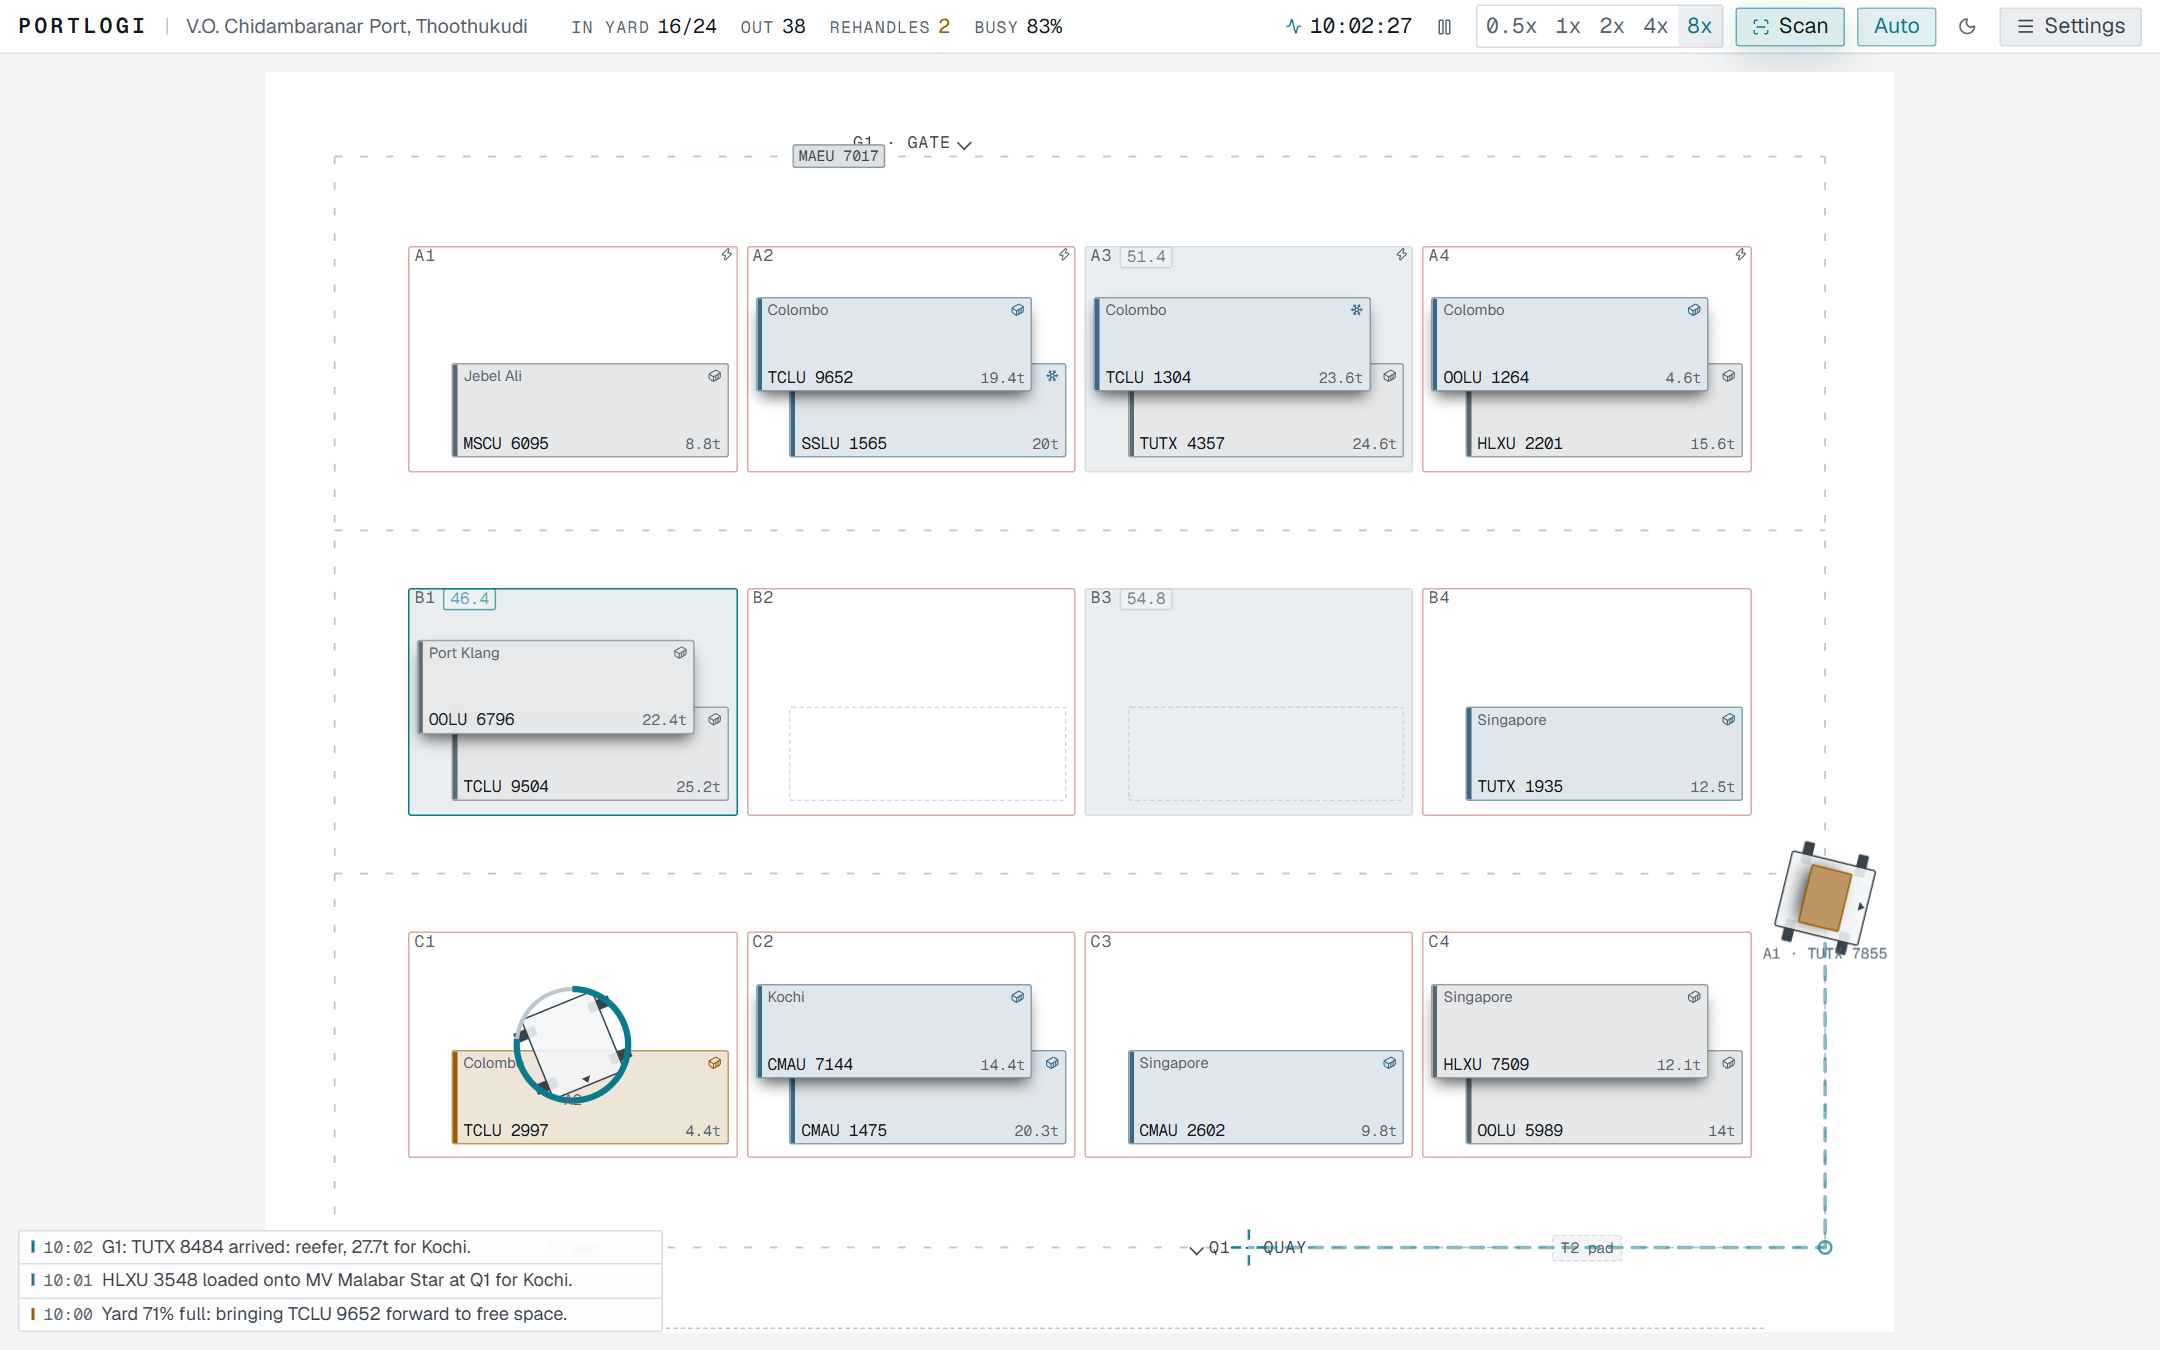
\includegraphics[width=\columnwidth]{fig/yard.png}
\caption{The yard view during a run. Boxes show their destination and weight. A vehicle is moving a box.}
\label{fig:yard}
\end{figure}

\begin{figure}[t]
\centering
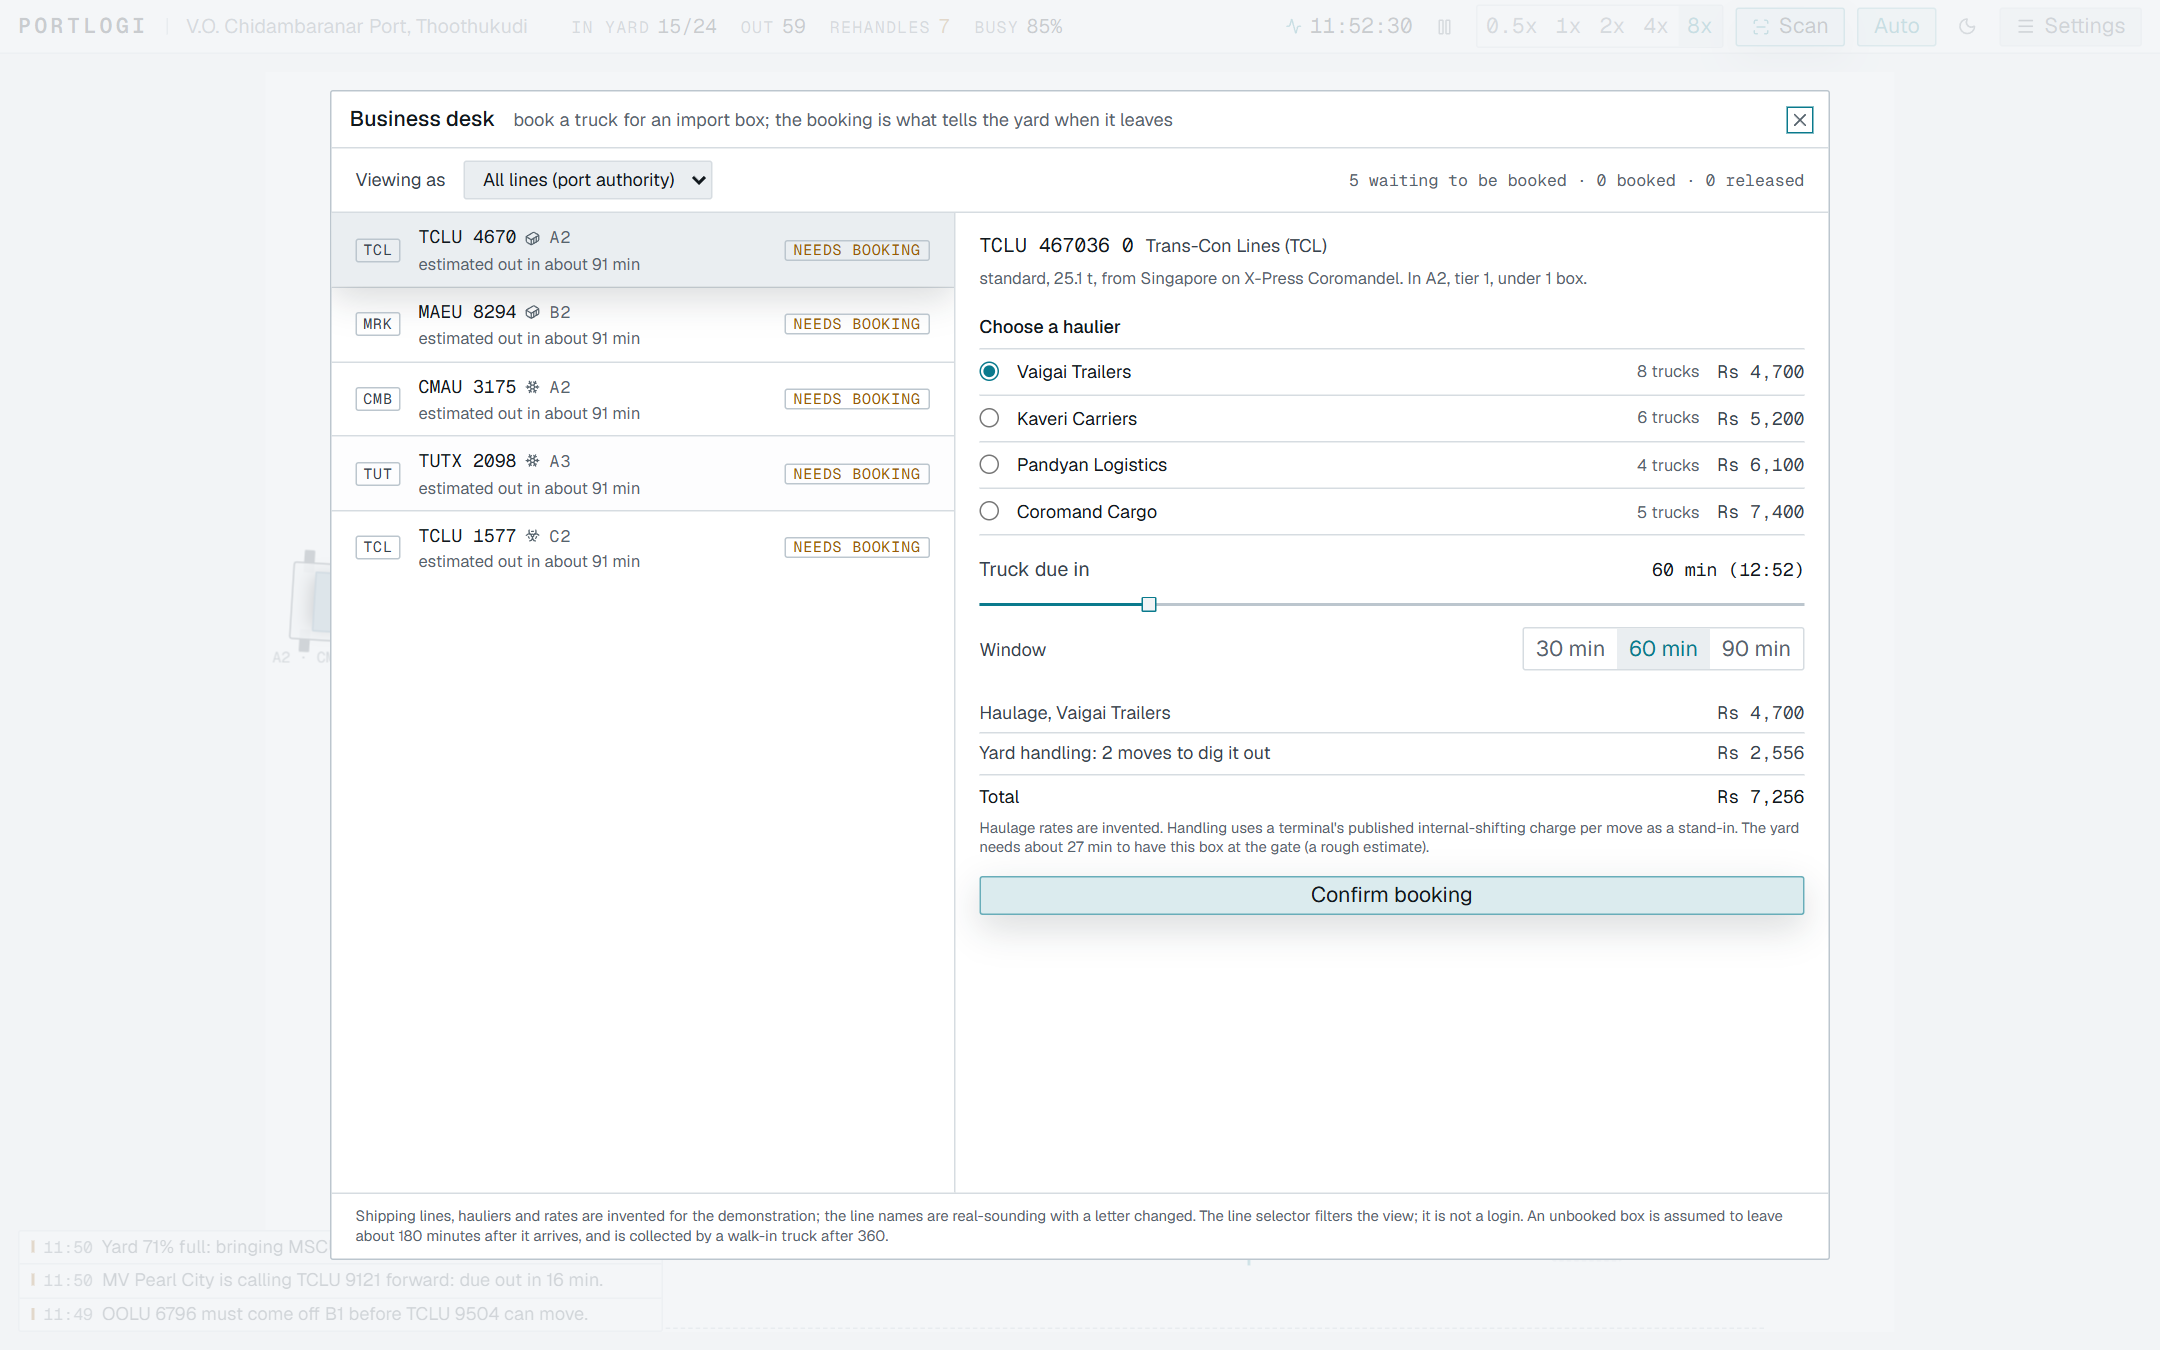
\includegraphics[width=\columnwidth]{fig/desk.png}
\caption{The business desk. A shipping line picks a haulier and a window and sees a quote.}
\label{fig:desk}
\end{figure}

\section{Results and Discussion}
All results come from the simulator. Unless stated, the yard has 3 rows, 4 columns, 2 tiers and 2 vehicles. Values are mean $\pm$ 95\% confidence interval.

\subsection{Placement quality}
We ran 100 seeds with 30 arrivals each. The same containers were used under both methods. Table~\ref{tab:head} shows the result. Rehandles fell by 69.6\%. The allocator was better in 96 runs, tied in 2 and worse in 2. No safety rule was broken in all 200 runs.

\begin{table}[t]
\caption{Allocator against first available placement (100 seeds)}
\label{tab:head}
\centering
\small
\begin{tabular}{lcc}
\toprule
Measure & First available & Allocator \\
\midrule
Rehandles per run & $6.7\pm0.4$ & $2.0\pm0.3$ \\
Grid cells driven & $917\pm10$ & $864\pm9$ \\
Time to clear (min) & $355\pm7$ & $345\pm6$ \\
Average dwell (min) & $112\pm2$ & $108\pm2$ \\
\bottomrule
\end{tabular}
\end{table}

First available is a weak baseline, so we also tested against a rule that uses departure time alone (the rehandle term only). Over 60 seeds, that rule gave 3.12 rehandles per run and the full allocator gave 2.15, which is about 31\% fewer. The simple departure time rule delivers about 80\% of the total gain. The other four terms add a smaller, steady gain.

\subsection{Ablation}
Table~\ref{tab:abl} turns off one term at a time (40 seeds). Removing the rehandle term hurts most (7.1 rehandles, no better than first available at 7.0). The other terms matter less, and removing aisle access costs the most among them.

\begin{table}[t]
\caption{One term removed at a time (40 seeds)}
\label{tab:abl}
\centering
\small
\begin{tabular}{lcc}
\toprule
Setting & Rehandles & Time to clear (min) \\
\midrule
All terms & $2.0\pm0.4$ & $342\pm9$ \\
Rehandle term only & $2.9\pm0.5$ & $355\pm11$ \\
No rehandle term & $7.1\pm0.6$ & $346\pm10$ \\
No travel & $1.9\pm0.5$ & $343\pm9$ \\
No cluster & $2.2\pm0.4$ & $342\pm10$ \\
No spread & $2.1\pm0.4$ & $344\pm9$ \\
No aisle access & $2.4\pm0.4$ & $348\pm11$ \\
First available & $7.0\pm0.5$ & $353\pm11$ \\
\bottomrule
\end{tabular}
\end{table}

\subsection{Bigger yards}
Table~\ref{tab:scale} shows four sizes, 12 seeds each. The gap grows with size. At 60 positions the allocator needed 7.1 rehandles and first available needed 56.7. A run of 60 positions takes about 1.6 seconds to simulate.

\begin{table}[t]
\caption{Scaling with yard size (12 seeds)}
\label{tab:scale}
\centering
\small
\begin{tabular}{lccc}
\toprule
Layout & Vehicles & Allocator & First avail. \\
\midrule
3x4 (12) & 2 & $0.9\pm0.4$ & $5.3\pm1.2$ \\
4x6 (24) & 4 & $2.8\pm0.9$ & $22.8\pm2.2$ \\
5x8 (40) & 5 & $5.7\pm1.7$ & $36.7\pm3.4$ \\
6x10 (60) & 6 & $7.1\pm1.6$ & $56.7\pm3.1$ \\
\bottomrule
\end{tabular}
\end{table}

\subsection{Fleet size}
On the small yard, one vehicle needed 371 minutes to clear the yard and kept gate waits near 12 minutes. Two vehicles cut that to 337 minutes and 5.2 minutes. A third vehicle helped little (334 minutes and 3.7 minutes) and was idle most of the time (utilisation 0.27).

\subsection{What is a pickup time worth?}
This experiment uses 20 import boxes and 32 seeds. The true pickup time is hidden and is drawn between 1 and 5 hours after arrival. We changed what the yard knows and when it learns it. The 1 to 5 hour range is our own choice, so the size of the effect is only an example. The pattern is the useful part.

\begin{table}[t]
\caption{Value of pickup time information (20 imports, 32 seeds)}
\label{tab:info}
\centering
\small
\begin{tabular}{lcc}
\toprule
What the yard knows & Rehandles & Truck wait (min) \\
\midrule
Guess only & $4.1\pm0.5$ & $9.8\pm3.1$ \\
Estimate, 60 min off & $3.1\pm0.4$ & $8.5\pm2.3$ \\
Estimate, 15 min off & $1.7\pm0.4$ & $7.2\pm1.9$ \\
Booked 20 min ahead & $4.0\pm0.5$ & $0.0\pm0.0$ \\
Booked 1 hour ahead & $4.0\pm0.5$ & $0.0\pm0.0$ \\
Booked 2 hours ahead & $3.8\pm0.4$ & $0.1\pm0.1$ \\
Booked at arrival & $1.3\pm0.4$ & $0.0\pm0.0$ \\
\bottomrule
\end{tabular}
\end{table}

\begin{figure}[t]
\centering
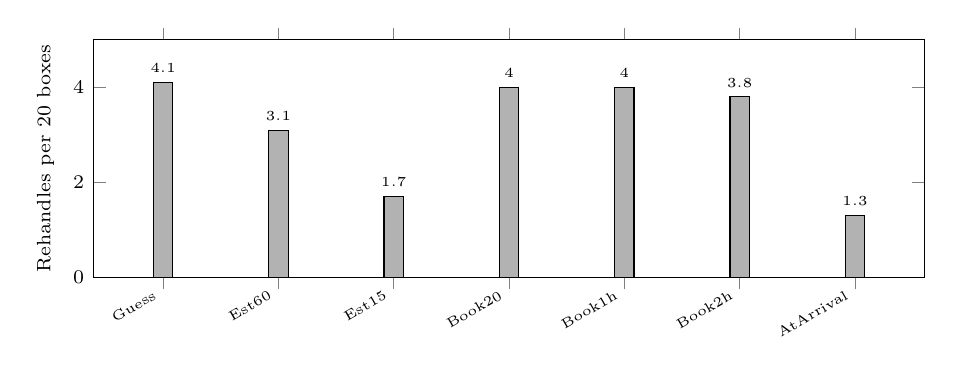
\begin{tikzpicture}
\begin{axis}[ybar, width=\columnwidth, height=4.6cm, bar width=7pt, ymin=0, ymax=5, ylabel={Rehandles per 20 boxes}, ylabel style={font=\scriptsize}, symbolic x coords={Guess,Est60,Est15,Book20,Book1h,Book2h,AtArrival}, xtick=data, x tick label style={font=\tiny, rotate=30, anchor=east}, tick label style={font=\scriptsize}, nodes near coords, nodes near coords style={font=\tiny}, enlarge x limits=0.1]
\addplot[fill=gray!60] coordinates {(Guess,4.1) (Est60,3.1) (Est15,1.7) (Book20,4.0) (Book1h,4.0) (Book2h,3.8) (AtArrival,1.3)};
\end{axis}
\end{tikzpicture}
\caption{Rehandles by what the yard knows. Only information known at placement helps.}
\label{fig:info}
\end{figure}

Two points stand out. First, a booking made 20 minutes to 2 hours before pickup does not lower rehandles (4.0 and 3.8 against 4.1). By then the box is already stacked. Only a time known at arrival cuts them, to 1.3. A good estimate (15 minutes off) also cuts them, to 1.7, without a firm booking. Second, any booking removes truck waiting, from about 10 minutes to almost none, because the yard has time to dig the box out and stage it. So the useful rule for a port authority is to ask for the booking when the box is discharged, not when the truck is about to leave.

\subsection{Safety, repeatability and tests}
We built 200 random yards (1 to 6 rows, 2 to 10 columns, 1 to 4 tiers, 1 to 6 vehicles, and a closed slot in 40\% of them). Each ran for 1000 simulated minutes with a vessel surge, a vehicle breakdown and a reefer storm. We found no collision, no illegal stack and no lost or doubled box, and no yard stalled. Ten seeds were run twice and gave identical states. The code has 108 unit tests and 12 tests for the web handler, and all pass. A separate test runs each of the 17 port yards for four simulated hours and checks the safety rules.

\subsection{Security}
The live site scored A+ on the Security Headers scan and A+ on all six server addresses in the SSL Labs test (both on 15 October 2026). Our own script passes 31 of 31 checks. These checks cover the policy headers, secure transport, blocked path tricks and file type handling. We do not claim the site is unbreakable. It holds no real port data.

\subsection{What it could save}
The booking desk and an impact calculator turn the result into money, using the published internal shifting charge of a terminal (INR 1,278 per move) as a stand-in for the value of one move. As an example only, take VOC Port at 734,274 TEU a year and 1.5 TEU per box, which gives about 489,500 boxes. The real rehandle rate of the port is not public, so assume 10\%. That is about 48,950 rehandles. A 31\% cut would avoid about 15,170 moves, worth about INR 1.94 crore a year. This is a what-if, not a measurement.

\subsection{Limits}
All results come from a simulator and a small yard. The real layout and rehandle rate of VOC Port are not public, so the other port yards are made up. Time is compressed, so dwell in the model is far shorter than in real life. The vehicle in the model both carries and stacks, which is closest to a straddle carrier. Our first available baseline is weak, which is why we also report the 31\% figure. The hardware gate is not built.

\section{Smart City Relevance}
\textbf{Citizens and businesses.} Shorter truck waits mean less idling near the port and less traffic on the roads to it. Small businesses get the same booking desk as large ones. These benefits are expected from the simulation, and we have not measured them in a real port.

\textbf{Sustainability.} Fewer wasted moves should mean less fuel or electricity per box. We did not measure energy.

\textbf{SDGs.} The work links to SDG 9 (industry, innovation and infrastructure), SDG 11 (sustainable cities), SDG 12 (responsible consumption and production) and SDG 13 (climate action).

\textbf{Scale.} The same engine runs yards from 12 to 60 positions. The landing page shows 17 ports, so the idea can be shown across a coast. A real roll out would need the real yard data and links to national port systems.

\section{Conclusion and Future Work}
Portlogi shows in simulation that a departure aware allocator with safe vehicle control cuts rehandles, and that a booking desk helps most when the booking comes at discharge. Next steps are to build and test the RFID gate, to feed the allocator forecasts of pickup time, and to test with real yard data.

\begin{thebibliography}{99}
\bibitem{dekker2006} R. Dekker, P. Voogd and E. van Asperen, ``Advanced methods for container stacking,'' \emph{OR Spectrum}, vol. 28, no. 4, pp. 563-586, 2006, doi: 10.1007/s00291-006-0038-3.
\bibitem{ku2016} D. Ku and T. S. Arthanari, ``Container relocation problem with time windows for container departure,'' \emph{European Journal of Operational Research}, vol. 252, no. 3, pp. 1031-1039, 2016, doi: 10.1016/j.ejor.2016.01.055.
\bibitem{caserta2012} M. Caserta, S. Schwarze and S. Vo{\ss}, ``A mathematical formulation and complexity considerations for the blocks relocation problem,'' \emph{European Journal of Operational Research}, vol. 219, no. 1, pp. 96-104, 2012.
\bibitem{galle2017} V. Galle, S. Borjian Boroujeni, V. H. Manshadi, C. Barnhart and P. Jaillet, ``The stochastic container relocation problem,'' arXiv:1703.04769, 2017.
\bibitem{mohring2005} R. H. M\"ohring, E. K\"ohler, E. Gawrilow and B. Stenzel, ``Conflict-free real-time AGV routing,'' in \emph{Operations Research Proceedings 2004}, Springer, 2005, pp. 18-24.
\bibitem{kim2007} K. H. Kim, S. M. Jeon and K. R. Ryu, ``Deadlock prevention for automated guided vehicles in automated container terminals,'' in \emph{Container Terminals and Cargo Systems}, K. H. Kim and H.-O. G\"unther, Eds. Springer, 2007, pp. 243-263, doi: 10.1007/978-3-540-49550-5\_12.
\bibitem{kaleris2023} Kaleris, ``Terminal Darsena Toscana solves yard planning challenges,'' case study, June 2023. [Online]. Available: \url{https://kaleris.com/?p=14697}
\bibitem{bw2024} ``Volume, productivity improved at most Indian ports in Q1-2024: S\&P,'' \emph{BusinessWorld}, 2024. [Online]. Available: \url{https://businessworld.in/article/volume-productivity-improved-at-most-indian-ports-in-q1-2024-sp-520277}
\bibitem{ldb} ``DMICDC launches pan-India Logistics Data Bank,'' \emph{Maritime Gateway}. [Online]. Available: \url{https://www.maritimegateway.com/dmicdc-launches-pan-india-logistics-data-bank/}
\bibitem{wikivoc} ``V. O. Chidambaranar Port,'' Wikipedia. [Online]. Available: \url{https://en.wikipedia.org/wiki/V._O._Chidambaranar_Port} (accessed Oct. 2026).
\bibitem{osm} OpenStreetMap contributors, map data and tiles. [Online]. Available: \url{https://www.openstreetmap.org/copyright}
\end{thebibliography}

\end{document}
